\documentclass{article}
\usepackage{amsmath}
\usepackage{tikz}

% Define the size of the diagram
\newcommand{\diagramSize}{6}
\newcommand{\numRows}{5}
\newcommand{\topRow}{5 4 3 1 0 0}
\newcommand{\bottomRow}{4 0 1 5 3 0}

\begin{document}

\section*{Multiline Diagram $D$}

A multiline diagram $D$ with \( n = 6 \) columns and \( s = 5 \) rows, with content \(\lambda = (5, 4, 3, 1, 0, 0)\) and bottom row \(\rho^{(1)}(D) = (4, 0, 1, 5, 3, 0) \in S_\lambda\). It has weight \(\wt(D) = \wt_x(D) \wt_t(D) = x_1^3 x_3^2 x_4^4 x_5^2 x_6^2 \, t^2\).

\begin{center}
    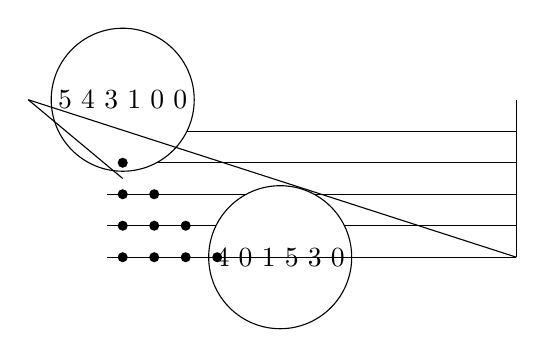
\begin{tikzpicture}[scale=0.8]
        \def\x{0.5} % Spacing between columns
        \def\y{0.5} % Height of each box
        
        % Draw horizontal lines
        \foreach \row in {1,...,\numRows}{
            \draw (\x/2, -\row*\y) -- (\diagramSize+1.5*\x, -\row*\y);
        }
        
        % Draw circles and numbers
        \foreach \col [count=\i] in {\topRow}{
            \node[circle, draw, fill=white, inner sep=2pt] at (\x*\i, 0) {\col};
        }
        
        % Draw circles and numbers in the bottom row
        \foreach \col [count=\i from \numRows+1] in {\bottomRow}{
            \node[circle, draw, fill=white, inner sep=2pt] at (\x*\i, -\numRows*\y) {\col};
        }
        
        % Draw diagonal lines
        \draw (-1, 0) -- (\diagramSize + 1.5 * \x, -\numRows * \y);
        \draw (\diagramSize + 1.5 * \x, 0) -- (\diagramSize + 1.5 * \x, -\numRows * \y);
        \draw (\x, -\numRows * \y) -- (\diagramSize + 1.5 * \x, -\numRows * \y);
        \draw (-1, 0) -- (\x, -\numRows * \y/2);
        \draw (\diagramSize + 1.5 * \x, 0) -- (\diagramSize + 1.5 * \x, -\numRows * \y/2);
        
        % Draw dots in between
        \foreach \col in {1, ..., \numRows}{
            \foreach \row in {1, ..., \numRows}{
                \ifnum\row>\col
                    \fill[black] (\x*\col, -\row*\y) circle (0.08);
                \fi
            }
        }
    \end{tikzpicture}
\end{center}

\end{document}